%!TEX root = ./main.tex



In this document we will be looking exclusively at physical systems with crystalline structure, or discrete translational symmetry. We will examine the consequences of such a symmetry in two cases. In the first case we look at continuous systems, where position space is a smooth manifold.  Next we will look at tight-binding models, where position space has been discretised into a lattice of sites. In both cases we see that in a system with crystalline structure the states are required to adhere to a band structure, and we will discuss the topology of this structure. We then describe some further consequences of periodic symmetry, introducing the definition of the Wannier states. \par

\subsection{Bloch's Theorem}
We start by examining the effect of discrete translational symmetry on a continuous system, the discussion is brief, a more comprehensive explanation can be found in \cite{simon_oxford_2013}. In such a system we obtain the energy eigenstates by solving Schrodinger's equation, which may be written in the position basis as
\begin{align}
     \hat H \psi(\bf x) = E \psi (\bf x),
\end{align}
where
\begin{align}
    \hat H = -\frac{\hbar^2}{2m}\nabla_{\bf{x}}^2 + V(\bf{x} ).
\end{align}
For the system to have crystalline structure we require that the potential $V(\bf x)$ is periodic in space, ensuring that
\begin{align}
    V(\bf x + \bf R) = V(\bf x),
\end{align}
for any vector $\bf R$ that lies on the Bravais lattice. \par
Bloch's Theorem, justified in Appendix \ref{appendix:bloch_proof}, states that the eigenstates of such a Hamiltonian can be expressed in the following form,
\begin{align}\label{eqn:bloch_states}
    \psi_{\bf k ,n }(\bf{x} )  = e^{i\bf{k}\cdot \hat{\bf{x}}}  u_{\bf k ,n }(\bf{x} ) ,
\end{align}
where $\bf k$ is a wave vector that lies in the first Brioullin zone and the state $u_{\bf k ,n }(\bf{x} )$ is periodic on the unit cell. In general we will have as many solutions for $u$ as there are bands in the material, the index $n$ labels which band a state belongs to. The form of the $u$-states is found by solving for the eigenstates of the bulk Hamiltonian
\begin{align}\label{eqn:bulk_hamiltonian}
    \hat H(\bf{k}) = e^{-i \bf{k} \cdot \hat{\bf{x}}} \hat H e^{i \bf{k} \cdot \hat{\bf{x}}},
\end{align}
obtained by substituting the Bloch ansatz into the Schrodinger equation. This Hamiltonian can be solved for states restricted to the unit cell with periodic boundaries.

\subsubsection{Lattice Models}\label{sec:lattice_bloch}
In a discrete system, we have a lattice of unit cells. We will label each cell by a set of numbers $\bf{m} = (m_1,m_2, ... , m_d)$, $m_i \in \mathbb{Z}$, where $d$ is the dimensionality of the material. Within each unit cell is a number $\eta$ of sites. Thus we can represent sites in our system as
\begin{align}
    \ket{\psi} = \ket{\bf m} \otimes \ket{\alpha}.
\end{align}
where $\bf m$ labels the unit cell and $\alpha \in \{1, 2 , ... , \eta\}$ labels the sites within the cell. States live in a Hilbert space with two subspaces
\begin{align}
    	\mathcal{H} = \mathcal{H}_{\textup{ext}} \otimes \mathcal{H}_{\textup{int}}
\end{align}
where the $\ket{\bf{m}}$ sites inhabit $\mathcal{H}_{\textup{ext}} $ and the $\ket{\alpha}$ sites inhabit $\mathcal{H}_{\textup{int}}$.\par
For the system to have lattice-translational symmetry, we require that the Hamiltonian respects translational invariance in $\mathcal{H}_{\textup{ext}}$. This means that we require the Hamiltonian, $\hat H$, to  obey
\begin{align}\label{eqn:lattice_trans}
    \braket{\bf m |\hat H| \bf n } = \braket{\bf m  + \bf L|\hat H| \bf n + \bf L}
\end{align}
for any $\bf m$, $\bf n $ and $\bf L \in \mathbb{Z} $.\par
Here we define the plane-wave basis $\ket {\bf k}$ according to
\begin{align}
	\ket{\bf k} = \frac{1}{\sqrt N} \sum_{\bf m} e^{i \bf m \cdot \bf k} \ket {\bf m},
\end{align}
where $N$ is the total number of unit cells in the system. If the Hamiltonian obeys equation \ref{eqn:lattice_trans}, then it can be diagonalised in the plane-wave basis. Thus our Hamiltonian can be re-expressed as
\begin{align}
	\hat H = \sum_{\bf k} \ket{\bf k} \bra{\bf k} \otimes \braket{\bf k | \hat H  | \bf k},
\end{align}
where we will label $\braket{\bf k |\hat  H  | \bf k}  = \hat H(\bf k)$, the bulk Hamiltonian. The tight-binding version of the bulk Hamiltonian acts on an $\eta$-dimensional Hilbert space -- since it is restricted to acting on states in a single unit cell -- and so has $\eta$ eigenvalues. Each of these eigenstates lives in a different band. From this it is clear to see that eigenstates of $\hat H$ take the form
\begin{align}
	\ket {\psi_{\bf k, n}} = \ket{\bf k} \otimes \ket{u_{\bf k, n}}.
\end{align}
Here, $\bf k$ represents a point in the first Brillouin zone and $n$ labels which of the $\eta$ solutions of $\hat H(\bf k)$ we are referring to, i.e. which band the state is in.

\subsubsection{Boundary Conditions}

Here it is worth mentioning the types of boundary conditions we will encounter, and commenting on the effect this has on the bloch states in a system. We will be mostly working in periodic boundary conditions, meaning that our lattice has some finite size in each dimension given by $(L_1,L_2, ... , L_d)$. Here the total number of unit cells in the system will be
\begin{align}
	N = \prod_{n=1}^{d}L_n.
\end{align}
If this is the case, the Brillouin zone will be discretised into a lattice of sites indexed by
\begin{align}
	\bf k = (\frac{2\pi}{L_1}a_1, \frac{2\pi}{L_2}a_2 , ... \frac{2\pi}{L_d} a_d),
\end{align}
where every number $a_i$ represents an integer in the interval $[0,L_i-1]$.\par
In the limit of an infinitely large system, the steps between discrete points in the lattice will become infinitesimal and the Brillouin zone becomes a smooth, closed manifold.

\subsubsection{A Note on Band Structure}
We comment briefly on the structure of these solutions. In both the continuous and lattice cases we have separated the eigenstates into two parts: a plane wave labelled by $\bf k$, which lives in the first Brillouin zone; and a state $\ket {u_{\bf k, n}}$ that is periodic with the unit cell, obtained by diagonalising the bulk Hamiltonian. Since the Brillouin Zone is generally a smooth, closed manifold, for each band (or value of $n$) we have effectively obtained a mapping from every point in the Brillouin zone to a state in the Hilbert space of states that are periodic with the unit cell. It is the topological characteristics of this mapping that will be of central importance in the discussion that follows, this will be expanded on in~\textsection\ref{sec:chern_number}. 

\begin{center}
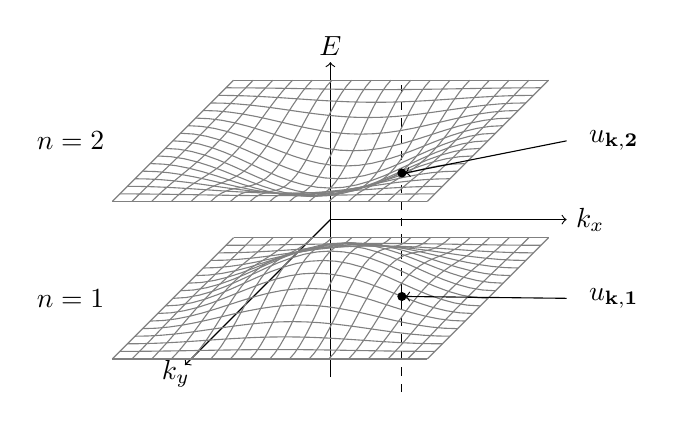
\begin{tikzpicture}

\def \size{3}
\def \vsize {2}
\def \ksize{2}
\def \stepnum {8}

\draw [->] (0,0) -- (\size,0,0);
\draw  [->] (0,-\vsize,0) -- (0,\vsize,0);
\draw  [->] (0,0) -- (0,0,1.6*\size);

\draw node at (1.1*\size,0,0) {$k_x$};
\draw node at (0,1.1*\vsize,0) {$E$};
\draw node at (0,0,1.7*\size) {$k_y$};

\draw node at (-1.1*\size , 1, 0) {$n=2$};
\draw node at (-1.1*\size , -1, 0) {$n=1$};

\def \xone {0.5}
\def \yone {1.1}

\draw [dashed] (\yone, -2 ,\xone) -- (\yone, 2 ,\xone);



\foreach \yy in {-\stepnum, ..., \stepnum}
{	
	\def \y {\yy*(\ksize/\stepnum)}
	\draw [domain = -\ksize:\ksize, variable= \x, gray] plot ({\y},{0.15*(1+cos(\x*360/(2*\ksize)))*(1+cos(\y*360/(2*\ksize))) -1},{\x});
	\draw [domain = -\ksize:\ksize, variable= \x, gray] plot ({\x},{0.15*(1+cos(\x*360/(2*\ksize)))*(1+cos(\y*360/(2*\ksize))) -1},{\y});
	
	\draw [domain = -\ksize:\ksize, variable= \x, gray] plot ({\y},{-0.15*(1+cos(\x*360/(2*\ksize)))*(1+cos(\y*360/(2*\ksize))) +1},{\x});
	\draw [domain = -\ksize:\ksize, variable= \x, gray] plot ({\x},{-0.15*(1+cos(\x*360/(2*\ksize)))*(1+cos(\y*360/(2*\ksize))) +1},{\y});
}


\draw[fill] ({\yone},{0.15*(1+cos(\xone*360/(2*\ksize)))*(1+cos(\yone*360/(2*\ksize))) -1},{\xone}) circle [radius=0.05];
\draw[fill] ({\yone},{-0.15*(1+cos(\xone*360/(2*\ksize)))*(1+cos(\yone*360/(2*\ksize)))+1},{\xone}) circle [radius=0.05];

\draw [->] (3,-1,0) --  ({\yone+0.04},{0.15*(1+cos(\xone*360/(2*\ksize)))*(1+cos(\yone*360/(2*\ksize))) -1},{\xone}) ;
\draw [->] (3,1,0) -- ({\yone+0.04},{-0.15*(1+cos(\xone*360/(2*\ksize)))*(1+cos(\yone*360/(2*\ksize))) +1},{\xone}) ;

\draw node at (1.2*\size,-1,0) {$\ket{u_{\bf k, 1}}$};
\draw node at (1.2*\size,1,0) {$\ket{u_{\bf k, 2}}$};


\end{tikzpicture}
\end{center}

This diagram shows the example for a system with two distinct bands, shown as the grey mesh plots. At each point in the bands there exists a corresponding $\ket{u_{\bf k , n}}$ state. 



\subsection{Wannier States}\label{sec:wannier_states}
Using Bloch's theorem, we have shown that it is straightforward to construct a set of energy eigenstates, separated into bands. These eigenstates are tightly localised in Fourier space, and so must as a result be delocalised across the whole system in real space. For each band in our system we have a set of states covering the whole of $k$-space. Thus it seems natural to ask whether these states can be combined to produce a basis of states that are delocalised in Fourier space, but localised in real space. Such states are called Wannier states, a  comprehensive review of these states may be found in \cite{marzari_maximally_2012}. \par
For each band, a set of Wannier states may be constructed by taking the Fourier transform of the complete set of energy eigenstates in that band, according to
\begin{align}
	\ket{w_{\bf R, n}} = \frac{V_{\textup{u.c.}}}{(2 \pi)^d } \int _{\textup{BZ}} d\bf k\; e^{-i \bf k \cdot \bf R + i \alpha(\bf k)} \ket{\psi _{\bf k, n}},
\end{align}
where $ V_{\textup{u.c.}}$ is the volume of the unit cell, $\bf R$ denotes a vector in the Bravais lattice, and $\alpha $ denotes an arbitrary gauge transformation that may be applied to the states. In practice, we usually work in systems with periodic boundaries. This means that the $\bf k$-states are restricted to lie on a lattice and the expression becomes
\begin{align}
	\ket{w_{\bf R, n}} = \frac{1}{\sqrt N } \sum _{\bf k}  e^{-i \bf k \cdot \bf R + i \alpha(\bf k)} \ket{\psi _{\bf k, n}}.
\end{align}
This construction represents a unitary transformation of the basis of energy eigenstates, thus the Wannier states also form an orthonormal complete basis set for the band. This means that the projector onto that band may be equivalently expressed in terms of Wannier states,
\begin{align}
	\hat P = \sum_{\bf k} \ket{\psi _{\bf k, n}}\bra{\psi _{\bf k, n}} \equiv \sum_{\bf R} \ket{w_{\bf R, n}} \bra{w_{\bf R, n}}.
\end{align}
Furthermore it can be shown that the states are related by translation,
\begin{align}
	\braket{\bf m | w_{\bf R, n} } = \braket{\bf m + \bf L | w_{\bf R + \bf L, n} },
\end{align}
for any lattice vector $\bf L$.\par
Although a gauge transformation does not have a measurable effect on the Bloch states, it does in fact have a strong effect on the Wannier states. This is because the choice of gauge allows us to control how localised our Wannier states are. If we are able to find a smooth gauge -- where $\ket{\psi_{\bf k, n}}$ is an analytic function of $\bf k$ -- we end up with a set of exponentially localised Wannier functions \cite{cloizeaux_energy_1964}. However if it is not possible to find a smooth gauge over the Brillouin zone, then we have an obstruction to finding a tightly localised set of Wannier states.\par
